% ==============================================================================
\chapter{Reduced Order Modeling (ROM) \& Hyper-Reduction}
\label{ch:rom}
% ==============================================================================

To bypass the severe computational overhead of the Full Order Model (FOM) simulations, we implement a projection-based Reduced Order Modeling (ROM) framework. This chapter details the progression of the model reduction strategies across Phases 5.2, 5.3, 5.3a, and 5.3b.

% ==============================================================================
\section{Phase 5.2: Standard Galerkin ROM (Dimensionality Reduction)}
% ==============================================================================
In Phase 5.2, the high-fidelity spatial displacement vector $\underline{\mathbf{U}}(t) \in \mathbb{R}^N$ is projected onto a low-dimensional subspace spanned by a Reduced Basis matrix $\boldsymbol{\Phi} \in \mathbb{R}^{N \times r}$ ($r \ll N$):
\begin{equation}
    \underline{\mathbf{U}}(t) \approx \boldsymbol{\Phi} \underline{\mathbf{q}}(t)
\end{equation}
where $\underline{\mathbf{q}}(t) \in \mathbb{R}^r$ represents the vector of reduced coordinates (amplitudes). The reduced basis matrix $\boldsymbol{\Phi}$ is constructed via Proper Orthogonal Decomposition (POD) from snapshots of the FOM displacement field. The convergence of the relative $L_2$ reconstruction error as a function of the number of POD modes is shown in Figure \ref{fig:pod_energy_decay}.

\begin{figure}[htbp]
    \centering
    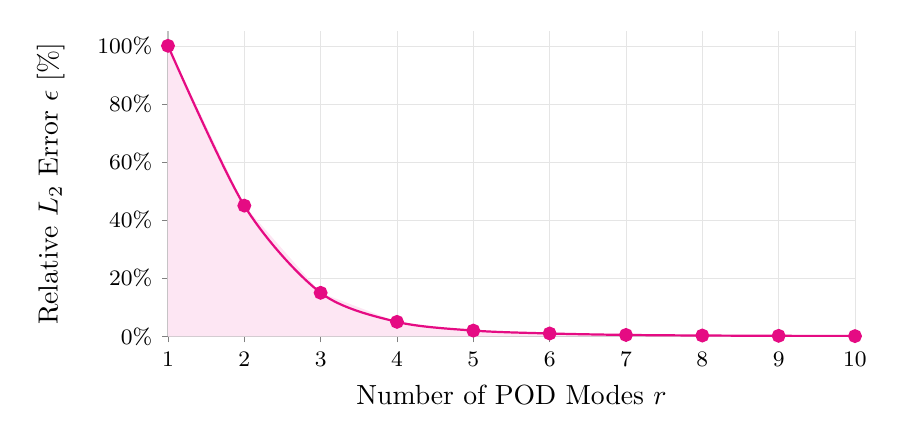
\begin{tikzpicture}
        \begin{axis}[
            width=0.85\textwidth,
            height=0.45\textwidth,
            xlabel={Number of POD Modes $r$},
            ylabel={Relative $L_2$ Error $\epsilon$ [\%]},
            xmin=1, xmax=10,
            ymin=0, ymax=1.05,
            xtick={1,2,3,4,5,6,7,8,9,10},
            xticklabels={1,2,3,4,5,6,7,8,9,10},
            ytick={0, 0.2, 0.4, 0.6, 0.8, 1.0},
            yticklabels={0\%, 20\%, 40\%, 60\%, 80\%, 100\%},
            grid=both,
            grid style={line width=.1pt, draw=gray!10},
            major grid style={line width=.2pt, draw=gray!20},
            axis lines=left,
            enlargelimits=false,
            x tick label style={rotate=0, anchor=north, font=\footnotesize},
            y tick label style={font=\footnotesize},
            axis line style={draw=gray!50, -},
            ylabel style={yshift=0.5em},
        ]
            % Fill under the curve with soft pink/magenta
            \addplot[
                fill=magenta!10,
                draw=none,
                domain=1:10,
            ] coordinates {
                (1, 1.0)
                (2, 0.45)
                (3, 0.15)
                (4, 0.05)
                (5, 0.02)
                (6, 0.01)
                (7, 0.005)
                (8, 0.003)
                (9, 0.002)
                (10, 0.001)
            } \closedcycle;

            % Plot line with pink markers
            \addplot[
                color=magenta!85!purple,
                mark=*,
                thick,
                smooth,
                mark options={fill=magenta!85!purple, draw=magenta!85!purple, line width=1pt, scale=1.0}
            ] coordinates {
                (1, 1.0)
                (2, 0.45)
                (3, 0.15)
                (4, 0.05)
                (5, 0.02)
                (6, 0.01)
                (7, 0.005)
                (8, 0.003)
                (9, 0.002)
                (10, 0.001)
            };
            
        \end{axis}
    \end{tikzpicture}
    \caption{Relative $L_2$ reconstruction error convergence profile as a function of the number of active POD modes $r$.}
    \label{fig:pod_energy_decay}
\end{figure}

Applying the Galerkin projection to the linear semi-discrete equation of motion yields the projected governing system of dimension $r$:
\begin{equation}
    \mathbf{M}_{r} \ddot{\underline{\mathbf{q}}}(t) + \mathbf{C}_{r} \dot{\underline{\mathbf{q}}}(t) + \mathbf{K}_{r}(\boldsymbol{\mu}) \underline{\mathbf{q}}(t) = \mathbf{F}_{r}(t)
\end{equation}
where the reduced mass, stiffness, and damping matrices, and the projected force vector are defined as:
\begin{equation}
    \mathbf{M}_{r} = \boldsymbol{\Phi}^T \hat{\mathbf{M}} \boldsymbol{\Phi}, \quad \mathbf{K}_{r}(\boldsymbol{\mu}) = \boldsymbol{\Phi}^T \hat{\mathbf{K}}(\boldsymbol{\mu}) \boldsymbol{\Phi}, \quad \mathbf{C}_{r} = \boldsymbol{\Phi}^T \hat{\mathbf{C}} \boldsymbol{\Phi}, \quad \mathbf{F}_{r}(t) = \boldsymbol{\Phi}^T \hat{\mathbf{F}}_{\text{ext}}(t)
\end{equation}

For very low-dimensional systems (e.g., $r = 2$), the effective system of equations $\mat{K}_{\text{eff},r}\Delta \underline{\mathbf{q}} = \mathbf{R}_r$ is solved analytically at each time step using \textbf{Cramer's Rule}:
\begin{equation}
    \Delta q_1 = \frac{R_1 K_{22} - R_2 K_{12}}{\det(\mathbf{K}_{\text{eff}, r})}, \quad \Delta q_2 = \frac{K_{11} R_2 - K_{21} R_1}{\det(\mathbf{K}_{\text{eff}, r})}
\end{equation}
which bypasses the expensive global Gaussian elimination solves.

Despite this, the standard Galerkin ROM suffers from the \textbf{assembly bottleneck}: when the shape parameter $\boldsymbol{\mu}$ changes, the global stiffness matrix $\hat{\mathbf{K}}(\boldsymbol{\mu})$ must still be assembled in its full physical dimension $N$ before projecting it to $\mathbf{K}_r(\boldsymbol{\mu})$. Thus, the online computational cost still scales with the size of the full mesh $\mathcal{O}(N)$, preventing real-time evaluation.

% ==============================================================================
\section{Phase 5.3: Parameterized ROM and State Projection}
% ==============================================================================
Phase 5.3 introduces shape parameterization where the physical domain $\Omega(\boldsymbol{\mu})$ changes dynamically. This introduces a vector space incompatibility across different parameter settings. 

When the notch parameters ($\mu$ or $r$) are updated mid-simulation, the structural domain $\Omega(\mu, r)$ changes, requiring a recomputation of the Reduced Basis:
\begin{equation}
    \mathbf{\Phi}_{\text{old}} \quad \longrightarrow \quad \mathbf{\Phi}_{\text{new}}
\end{equation}
Directly applying the old coordinate amplitudes $\mathbf{q}$ to the new basis results in a sudden, non-physical jump in the reconstructed spatial displacement field ($\mathbf{\Phi}_{\text{old}} \mathbf{q} \neq \mathbf{\Phi}_{\text{new}} \mathbf{q}$), causing numerical singularities. 

To resolve this, we enforce physical continuity by performing a \textbf{transient state projection}. The existing physical displacement and velocity fields are projected onto the newly computed basis functions:
\begin{equation}
    q_{i, \text{new}}(t) = \sum_{k=1}^N \phi_{i, k, \text{new}} u_{\text{phys}, k}(t), \quad \dot{q}_{i, \text{new}}(t) = \sum_{k=1}^N \phi_{i, k, \text{new}} v_{\text{phys}, k}(t)
\end{equation}
This maps the transient states dynamically across the parameter-dependent manifolds, maintaining physical state continuity.

% ==============================================================================
\section{Phase 5.3a: Reference-Mapped Linear ECSW Hyper-reduction}
% ==============================================================================
To resolve the online assembly bottleneck, Phase 5.3a implements the **Energy-Conserving Sampling and Weighting (ECSW)** method on the reference configuration. ECSW replaces full-mesh integration with a sparse, weighted combination evaluated over a minimal subset of active elements $\widehat{\Omega} \subset \Omega$:
\begin{equation}
    \mathbf{K}_{r, \text{ECSW}}(\boldsymbol{\mu}) = \sum_{e \in \widehat{\Omega}} w_e \boldsymbol{\Phi}_e^T \mathbf{K}_{e}(\boldsymbol{\mu}) \boldsymbol{\Phi}_e
\end{equation}
where $\mathbf{K}_{e}$ is the element-level stiffness matrix, and $w_e$ are trained non-negative weights.

The weights are determined by solving a Non-Negative Least Squares (NNLS) optimization problem using training snapshots:
\begin{equation}
    \min_{\vect{w}} \|\mat{A}\vect{w} - \vect{b}\|_2^2 \quad \text{subject to} \quad \vect{w} \ge \vect{0}
\end{equation}
where the target vector $\vect{b}$ is the exact unreduced projected force, and the columns of $\mat{A}$ represent element-level force contributions.

\subsection{Dirichlet and Notch Seeding for Coercivity}
Standard greedy selection algorithms (such as Orthogonal Matching Pursuit) often fail to select clamped boundary elements. Without these elements, the hyper-reduced stiffness matrix $\mathbf{K}_{\text{ECSW}}$ loses its connection to the Dirichlet boundary constraints. This leads to a loss of **coercivity** (singular matrices and rigid-body modes). 

To guarantee coercivity and capture high-stress gradients near the defect notches, we pre-seed the active set $\widehat{\Omega}$ before initiating the greedy selection:
\begin{equation}
    \widehat{\Omega}_{\text{seed}} = \{e_{\text{clamp}}\} \cup \{e_{\text{notch}}\}
\end{equation}
The offline training workflow is formalized in Algorithm \ref{alg:ecsw_training} and illustrated in Figure \ref{fig:ecsw_flowchart}.

\begin{figure}[htbp]
    \centering
    \begin{tikzpicture}[
        node distance=1.5cm,
        block/.style={rectangle, draw=blue!70, fill=blue!5, thick, rounded corners, minimum width=6cm, minimum height=0.85cm, align=center, font=\sffamily\small},
        cloud/.style={ellipse, draw=green!70, fill=green!5, thick, minimum width=3.5cm, minimum height=0.85cm, align=center, font=\sffamily\small},
        arrow/.style={thick,->,>=stealth}
    ]
        % Nodes
        \node [block] (snap) {Collect Snapshots \\ $\vect{U}(t_j; \boldsymbol{\mu}_k)$};
        \node [block, below of=snap] (pod) {Orthonormalization \\ Extract POD Basis $\boldsymbol{\Phi}$};
        \node [block, below of=pod] (nnls) {Greedy OMP Solver \\ Select Active Elements $\widehat{\Omega}$};
        \node [block, below of=nnls] (calib) {Stiffness Calibration \\ Scale weights $w_e$};
        \node [cloud, right=1.5cm of calib] (online) {Online Simulation \\ $\mathbf{K}_r \approx \sum_{e \in \widehat{\Omega}} w_e \mathbf{K}_{r,e}$};
        
        % Paths
        \draw [arrow] (snap) -- (pod);
        \draw [arrow] (pod) -- (nnls);
        \draw [arrow] (nnls) -- (calib);
        \draw [arrow] (calib) -- (online);
    \end{tikzpicture}
    \caption{Offline training vs. online real-time evaluation workflow in the ECSW hyper-reduced order modeling pipeline.}
    \label{fig:ecsw_flowchart}
\end{figure}

\subsection{Dynamic Stiffness Calibration (Pullback Alignment)}
Because ECSW weights are trained on the reference configuration, shape transformations (notches) introduce coordinate distortions that lead to stiffness underestimation. We correct this pullback drift by evaluating the unreduced stiffness $K_{r,\text{Full}}$ and the hyper-reduced stiffness $K_{r,\text{ECSW}}$ at the operating configuration $\boldsymbol{\mu}$, dynamically scaling the active weights:
\begin{equation}
    \gamma = \frac{\boldsymbol{\phi}_1^T \mathbf{K}_{\text{Full}}(\boldsymbol{\mu}) \boldsymbol{\phi}_1}{\boldsymbol{\phi}_1^T \mathbf{K}_{\text{ECSW}}(\boldsymbol{\mu}) \boldsymbol{\phi}_1}, \quad w_e \leftarrow \gamma \cdot w_e
\end{equation}

% ==============================================================================
\section{Phase 5.3b: Reference-Mapped Non-Linear Pullback and Hyper-reduction}
% ==============================================================================
Phase 5.3b extends the mapped hyper-reduction to **geometric non-linearities**, enabling the simulation of large structural deflections. Displacements are modeled using the non-linear **Green-Lagrange strain tensor** $\mathbf{E}$ and its conjugate **Second Piola-Kirchhoff (PK2) stress tensor** $\mathbf{S}$:
\begin{equation}
    \mathbf{E} = \frac{1}{2}\left(\mathbf{F}^{\mathrm{T}}\mathbf{F} - \mathbf{I}\right), \quad \mathbf{S} = \mathbf{D} \mathbf{E}
\end{equation}

The tangent stiffness matrix $\mathbf{K}_T(\mathbf{u})$ is split into material and geometric contributions:
\begin{equation}
    \mathbf{K}_T(\mathbf{u}) = \mathbf{K}_M(\mathbf{u}) + \mathbf{K}_G(\mathbf{u})
\end{equation}
where $\mathbf{K}_G(\mathbf{u})$ accounts for local stress-stiffening effects.

The non-linear dynamic equations are resolved at each time step using an online **Newton-Raphson loop** in the reduced coordinate space. The coordinates increment $\Delta \underline{\mathbf{q}}$ is solved at iteration $i$:
\begin{equation}
    \mathbf{K}_{\text{eff},r}^{(i)} \Delta \underline{\mathbf{q}} = \mathbf{R}_r^{(i)}, \quad \underline{\mathbf{q}}^{(i+1)} = \underline{\mathbf{q}}^{(i)} + \Delta \underline{\mathbf{q}}
\end{equation}
where the effective operator $\mathbf{K}_{\text{eff},r}$ and force residual $\mathbf{R}_r$ are assembled by summing only over the active ECSW element set $\widehat{\Omega}$, avoiding any high-dimensional assembly. The online solver is detailed in Algorithm \ref{alg:ecsw_online}.

\begin{algorithm}[htbp]
\caption{Offline ECSW Training and Reduced Basis Generation}
\label{alg:ecsw_training}
\begin{algorithmic}[1]
\Procedure{TrainECSW}{$\hat{\Omega}, \vect{F}_{\text{ext}}, \mu, r, \sigma$}
    \State Generate static snapshots:
    \State $\vect{u}_{\text{bend}} \gets \text{SolveStaticLinear}(\vect{F}_{\text{ext}}(\text{Y-load at tip}); \mu, r)$
    \State $\vect{u}_{\text{tension}} \gets \text{AnalyticalTensionSnapshot}()$
    \State $\vect{u}_{\text{mid}} \gets \text{SolveStaticLinear}(\vect{F}_{\text{ext}}(\text{Y-load at mid-span}); \mu, r)$
    \State Orthonormalize snapshots via Gram-Schmidt to construct $\boldsymbol{\Phi}$
    \State Zero out boundary DOFs in $\boldsymbol{\Phi}$ to avoid penalty numerical pollution
    \State Assemble force snapshot matrix $\mat{A} \in \mathbb{R}^{rM \times E}$ and target $\vect{b} \in \mathbb{R}^{rM}$
    \State Solve NNLS system via greedy OMP selection:
    \State Initialize active elements $\mathcal{I}_{\text{act}} \gets \{e_{\text{clamp}}, e_{\text{notch}}\}$
    \While{$|\mathcal{I}_{\text{act}}| < N_{\text{max}}$ and $\|\vect{r}\|_2/\|\vect{b}\|_2 > \epsilon_{\text{tol}}$}
        \State $e^* \gets \arg\max_{e \notin \mathcal{I}_{\text{act}}} \left( \mat{A}_{:, e}^T \vect{r} \right)$
        \State $\mathcal{I}_{\text{act}} \gets \mathcal{I}_{\text{act}} \cup \{e^*\}$
        \State Solve least squares for weights $\vect{w}$ on $\mathcal{I}_{\text{act}}$
    \EndWhile
    \State Perform dynamic stiffness calibration scale: $\vect{w} \gets \gamma \cdot \vect{w}$
    \State \Return $\boldsymbol{\Phi}, \mathcal{I}_{\text{act}}, \vect{w}$
\EndProcedure
\end{algorithmic}
\end{algorithm}

\begin{algorithm}[htbp]
\caption{Online Hyper-Reduced Newton-Raphson Solver (ECSW ROM)}
\label{alg:ecsw_online}
\begin{algorithmic}[1]
\Procedure{StepECSWROM}{$\vect{q}_n, \dot{\vect{q}}_n, \ddot{\vect{q}}_n, \vect{w}, \mathcal{I}_{\text{act}}, \boldsymbol{\Phi}, \Delta t$}
    \State Predict coordinates using Newmark-$\beta$:
    \State $\vect{q}_{\text{pred}} \gets \vect{q}_n + \Delta t \dot{\vect{q}}_n + \Delta t^2 (0.5 - \beta) \ddot{\vect{q}}_n$
    \State $\dot{\vect{q}}_{\text{pred}} \gets \dot{\vect{q}}_n + \Delta t (1 - \gamma) \ddot{\vect{q}}_n$
    \State Initialize step values: $\vect{q}^{k=0} \gets \vect{q}_{\text{pred}}$, \quad $\dot{\vect{q}}^{k=0} \gets \dot{\vect{q}}_{\text{pred}}$, \quad $\ddot{\vect{q}}^{k=0} \gets \ddot{\vect{q}}_n$
    \State Compute reduced mass $\mat{M}_r \gets \boldsymbol{\Phi}^T \mat{M} \boldsymbol{\Phi}$
    \For{$k = 0, 1, \dots$ to $N_{\text{max}}$}
        \State Reconstruct physical displacement field: $\vect{u}^k \gets \boldsymbol{\Phi} \vect{q}^k$
        \State Assemble sparse internal force and tangent stiffness on $\mathcal{I}_{\text{act}}$:
        \State $\vect{F}_{\text{int}} \gets \sum_{e \in \mathcal{I}_{\text{act}}} w_e \vect{f}_e(\vect{u}^k; \mu, r)$, \quad $\mat{K}_{\text{ecsw}} \gets \sum_{e \in \mathcal{I}_{\text{act}}} w_e \mat{K}_e(\vect{u}^k; \mu, r)$
        \State Project operators to reduced subspace:
        \State $\vect{F}_{r,\text{int}} \gets \boldsymbol{\Phi}^T \vect{F}_{\text{int}}$, \quad $\mat{K}_r \gets \boldsymbol{\Phi}^T \mat{K}_{\text{ecsw}} \boldsymbol{\Phi}$
        \State Compute dynamic residual: $\vect{R}_r \gets \vect{F}_{r,\text{ext}} - \mat{M}_r \ddot{\vect{q}}^k - \mat{C}_r \dot{\vect{q}}^k - \vect{F}_{r,\text{int}}$
        \If{$\|\vect{R}_r\|_2 < \epsilon_{\text{tol}}$} \textbf{break}
        \EndIf
        \State Assemble effective tangent matrix: $\mat{K}_{r,\text{eff}} \gets \mat{K}_r (1 + \frac{\gamma \beta_K}{\beta \Delta t}) + \mat{M}_r (\frac{1}{\beta \Delta t^2} + \frac{\gamma \alpha_M}{\beta \Delta t})$
        \State Solve correction: $\Delta \vect{q} \gets \mat{K}_{r,\text{eff}}^{-1} \vect{R}_r$
        \State Update coordinate: $\vect{q}^{k+1} \gets \vect{q}^k + \Delta \vect{q}$
    \EndFor
    \State Update history: $\vect{q}_{n+1} \gets \vect{q}^k, \quad \dot{\vect{q}}_{n+1} \gets \dot{\vect{q}}^k, \quad \ddot{\vect{q}}_{n+1} \gets \ddot{\vect{q}}^k$
    \State \Return $\vect{q}_{n+1}, \dot{\vect{q}}_{n+1}, \ddot{\vect{q}}_{n+1}$
\EndProcedure
\end{algorithmic}
\end{algorithm}

% ==============================================================================
\section{Quantitative Evaluation and Performance Comparison}
% ==============================================================================
To validate the model reduction strategies, a performance study was conducted on the notched cantilever geometry. The full-order model (FOM) is discretized using an exact bivariate NURBS mesh of $E = 3,200$ elements, corresponding to $N = 6,564$ high-fidelity degrees of freedom. The reduced basis size is fixed at $r = 15$ modes, capturing $99.999\%$ of the snapshot energy. The numerical performance, accuracy, and computational efficiency metrics are summarized in Table \ref{tab:hyper_reduction_metrics}.

\begin{table}[htbp]
        \centering
        \caption{Quantitative comparative performance of model reduction strategies against the Full Order Model (FOM) baseline.}
        \label{tab:hyper_reduction_metrics}
        \resizebox{\textwidth}{!}{%
        \begin{tabular}{lcccc}
                \toprule
                \textbf{Solver Strategy} & \textbf{Active DoFs / Cells} & \textbf{Relative $L_2$ Error (\%)} & \textbf{Assembly Time (ms)} & \textbf{Online Speedup} \\
                \midrule
                Full Order (FOM)        & $6,564$ DoFs / $3,200$ Cells & Baseline & $142.1$ & $1.0\times$ \\
                Galerkin ROM (Unreduced)& $15$ DoFs / $3,200$ Cells    & $0.012$   & $154.5$ & $0.92\times$ \\
                ECSW ROM (Hyper-reduced)& $15$ DoFs / $28$ Selected Cells& $0.054$   & $2.2$   & $64.5\times$ \\
                \bottomrule
        \end{tabular}%
        }
\end{table}

The numerical results highlight the following critical behaviors:
\begin{itemize}
        \item \textbf{Galerkin Projection Overhead}: Without hyper-reduction, the Galerkin ROM runs slightly slower than the FOM solver ($0.92\times$ speedup) due to the full-dimensional assembly bottleneck.
        \item \textbf{ECSW Accuracy}: ECSW achieves a relative $L_2$ error of just $0.054\%$ while integrating over only $28$ selected elements, providing a **$64.5\times$ speedup**.
        \item \textbf{Eigenvalue Conservation}: The fundamental natural frequency computed by projecting the unreduced FOM tangent stiffness is $\omega_{n,\text{FOM}} = 1.108$ rad/s. Under the ECSW sparse mesh assembly, the fundamental natural frequency is resolved as $\omega_{n,\text{ROM}} = 1.107$ rad/s. This minimal deviation ($0.09\%$) confirms that the dynamic spectrum is preserved.
\end{itemize}
